\chapter{第16套试卷——参考答案与评分标准}

\section{一、选择题答案（18分）}

\begin{enumerate}[label=\arabic*.]
\item \textbf{B} — CLB/Slice包含LUT、D触发器、MUX和进位链。
\item \textbf{B} — 信号(\texttt{<=})在进程挂起后更新；变量(\texttt{:=})立即生效。
\item \textbf{C} — 敏感列表不完整导致锁存器推断。
\item \textbf{A} — Moore输出仅取决于状态；Mealy取决于状态+输入。
\item \textbf{D} — 并发语句和顺序语句均可描述组合/时序逻辑。
\item \textbf{B} — NOT优先级最高，然后AND，最后OR。
\end{enumerate}

\section{二、填空题答案（12分）}

\begin{enumerate}[label=\arabic*.]
\item \textbf{（1）IEEE.STD\_LOGIC\_1164} \quad \textbf{（2）IEEE.NUMERIC\_STD}
\item \textbf{（1）<=} \quad \textbf{（2）:=}
\item GENERIC声明应在PORT声明\textbf{之前}
\item \textbf{（1）COMPONENT} \quad \textbf{（2）PORT MAP}
\end{enumerate}

\section{三、程序改错题解析（5分）}

\begin{enumerate}[label=错误\arabic*：]
\item 库引用错误：\texttt{STD\_LOGIC\_ARITH}应为\texttt{NUMERIC\_STD}，且缺少\texttt{STD\_LOGIC\_1164}。
\item 敏感列表缺少\texttt{en}信号。
\item CASE缺少\texttt{WHEN OTHERS}分支。
\item 漏分号：\texttt{Y <= "00010000"}后缺\texttt{;}。
\item PORT括号不匹配。
\end{enumerate}

\textbf{修正后代码：}
\begin{lstlisting}
library IEEE;
use IEEE.STD_LOGIC_1164.all;
use IEEE.NUMERIC_STD.all;

entity decoder_3to8 is
  port(
    A  : in  std_logic_vector(2 downto 0);
    en : in  std_logic;
    Y  : out std_logic_vector(7 downto 0)
  );
end decoder_3to8;

architecture behav of decoder_3to8 is
begin
  process(A, en)
  begin
    if en = '0' then Y <= (others => '0');
    else
      case A is
        when "000" => Y <= "00000001";
        when "001" => Y <= "00000010";
        when "010" => Y <= "00000100";
        when "011" => Y <= "00001000";
        when "100" => Y <= "00010000";
        when "101" => Y <= "00100000";
        when "110" => Y <= "01000000";
        when "111" => Y <= "10000000";
        when others => Y <= (others => '0');
      end case;
    end if;
  end process;
end behav;
\end{lstlisting}

{\centering 评分：每找出并正确修正1处得1分，共5分。\par}

\section{四、程序阅读分析题解析（5分）}

\textbf{（1）电路类型（1分）：}6分频器（模6计数器+输出逻辑）。\\
\textbf{（2）功能（1分）：}将clk进行6分频，$f_{out}=f_{clk}/6$。\\
\textbf{（3）占空比（1.5分）：}cnt=0,1,2时输出0；cnt=3,4,5时输出1。高电平3拍、低电平3拍，占空比\textbf{50\%}。\\
\textbf{（4）频率（1.5分）：}$f_{clk}=50\text{MHz}$时，$f_{out}=50/6\approx 8.33\text{MHz}$。

\section{五、综合设计题参考答案（60分）}

\subsection{设计题1：带使能的3-8译码器（20分）}

\textbf{【分析】}3-8译码器：3位输入→8位独热输出。en=1正常译码；en=0全0。

\textbf{【VHDL】}
\begin{lstlisting}
library IEEE;
use IEEE.STD_LOGIC_1164.all;

entity decoder_3to8_en is
  port(
    A  : in  std_logic_vector(2 downto 0);
    en : in  std_logic;
    Y  : out std_logic_vector(7 downto 0)
  );
end decoder_3to8_en;

architecture behav of decoder_3to8_en is
begin
  process(A, en)
  begin
    if en = '0' then Y <= (others => '0');
    else
      case A is
        when "000" => Y <= "00000001";
        when "001" => Y <= "00000010";
        when "010" => Y <= "00000100";
        when "011" => Y <= "00001000";
        when "100" => Y <= "00010000";
        when "101" => Y <= "00100000";
        when "110" => Y <= "01000000";
        when "111" => Y <= "10000000";
        when others => Y <= (others => '0');
      end case;
    end if;
  end process;
end behav;
\end{lstlisting}

\textbf{【评分】（20分）}ENTITY声明4分 + en=0逻辑4分 + CASE完整6分 + 独热编码4分 + 敏感列表2分。

\subsection{设计题2：模6计数器（20分）}

\textbf{【分析】}$N=6$，$k=\lceil\log_2 6\rceil=3$位，清零$cnt=5(101)$。

\textbf{【VHDL】}
\begin{lstlisting}
library IEEE;
use IEEE.STD_LOGIC_1164.all;
use IEEE.NUMERIC_STD.all;

entity counter_mod6 is
  port(
    clk   : in  std_logic;
    rst   : in  std_logic;
    count : out std_logic_vector(2 downto 0);
    tc    : out std_logic
  );
end counter_mod6;

architecture behav of counter_mod6 is
  signal cnt : unsigned(2 downto 0) := (others => '0');
begin
  process(clk, rst)
  begin
    if rst = '1' then cnt <= (others => '0');
    elsif rising_edge(clk) then
      if cnt = 5 then cnt <= (others => '0');
      else cnt <= cnt + 1; end if;
    end if;
  end process;
  count <= std_logic_vector(cnt);
  tc <= '1' when cnt = 5 else '0';
end behav;
\end{lstlisting}

\textbf{【评分】（20分）}分析(N=6,k=3)3分 + ENTITY 3分 + 异步复位3分 + cnt=5清零4分 + NUMERIC\_STD 3分 + tc信号2分 + 规范2分。

\subsection{设计题3：自动售货机控制器（20分）}

\textbf{【分析】}商品5元，硬币1元/2元。Moore型，7状态(S0=0元$\sim$S5=5元出货, S6=超5元找零)。

\textbf{【状态转移图】}
\begin{center}
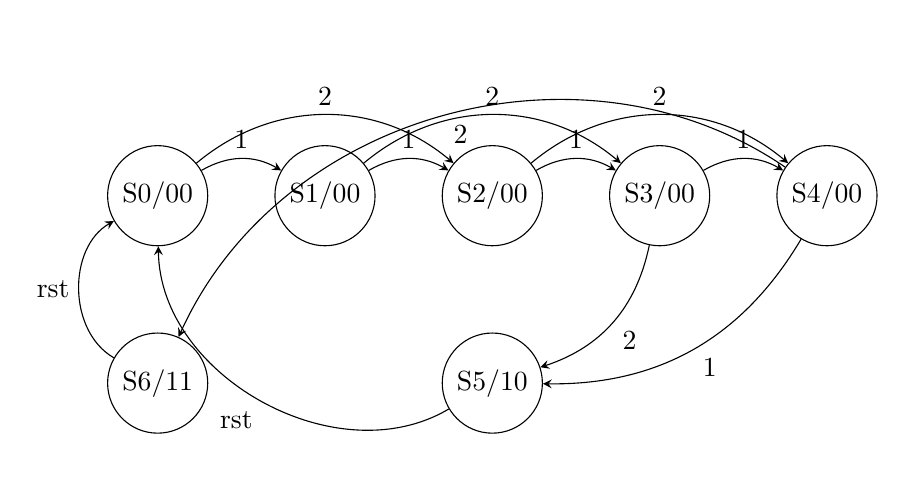
\begin{tikzpicture}[->,>=stealth,node distance=2.8cm,auto,scale=0.85]
\node[draw,circle] (S0) at (0,0) {S0/00};
\node[draw,circle] (S1) at (2.5,0) {S1/00};
\node[draw,circle] (S2) at (5,0) {S2/00};
\node[draw,circle] (S3) at (7.5,0) {S3/00};
\node[draw,circle] (S4) at (10,0) {S4/00};
\node[draw,circle] (S5) at (5,-2.8) {S5/10};
\node[draw,circle] (S6) at (0,-2.8) {S6/11};
\draw (S0) edge[bend left] node{1} (S1);
\draw (S1) edge[bend left] node{1} (S2);
\draw (S2) edge[bend left] node{1} (S3);
\draw (S3) edge[bend left] node{1} (S4);
\draw (S4) edge[bend left] node{1} (S5);
\draw (S0) edge[bend left=40] node{2} (S2);
\draw (S1) edge[bend left=40] node{2} (S3);
\draw (S2) edge[bend left=40] node{2} (S4);
\draw (S3) edge[bend left] node{2} (S5);
\draw (S4) edge[bend right=50] node{2} (S6);
\draw (S5) edge[bend left=60] node{rst} (S0);
\draw (S6) edge[bend left=60] node{rst} (S0);
\end{tikzpicture}
\end{center}
（注：弧上数字为投币面额，状态/输出格式为 dispense/change）

\textbf{【状态转移表】}
\begin{center}
\begin{tabular}{|c|c|c||c|c|}
\hline
当前 & 投1元 & 投2元 & dispense & change \\
\hline
S0(0元) & S1 & S2 & 0 & 0 \\
S1(1元) & S2 & S3 & 0 & 0 \\
S2(2元) & S3 & S4 & 0 & 0 \\
S3(3元) & S4 & S5 & 0 & 0 \\
S4(4元) & S5 & S6 & 0 & 0 \\
S5(5元) & S0 & S0 & 1 & 0 \\
S6(>5元) & S0 & S0 & 1 & 1 \\
\hline
\end{tabular}
\end{center}

\textbf{【VHDL】}
\begin{lstlisting}
library IEEE;
use IEEE.STD_LOGIC_1164.all;

entity vending_machine is
  port(
    clk      : in  std_logic;
    rst      : in  std_logic;
    coin_1   : in  std_logic;
    coin_2   : in  std_logic;
    dispense : out std_logic;
    change   : out std_logic
  );
end vending_machine;

architecture moore_fsm of vending_machine is
  type state_type is (S0, S1, S2, S3, S4, S5, S6);
  signal curr_state, next_state : state_type;
begin
  reg_proc: process(clk, rst)
  begin
    if rst = '1' then curr_state <= S0;
    elsif rising_edge(clk) then curr_state <= next_state;
    end if;
  end process;

  comb_proc: process(curr_state, coin_1, coin_2)
  begin
    case curr_state is
      when S0 =>
        if coin_2 = '1' then next_state <= S2;
        elsif coin_1 = '1' then next_state <= S1;
        else next_state <= S0; end if;
      when S1 =>
        if coin_2 = '1' then next_state <= S3;
        elsif coin_1 = '1' then next_state <= S2;
        else next_state <= S1; end if;
      when S2 =>
        if coin_2 = '1' then next_state <= S4;
        elsif coin_1 = '1' then next_state <= S3;
        else next_state <= S2; end if;
      when S3 =>
        if coin_2 = '1' then next_state <= S5;
        elsif coin_1 = '1' then next_state <= S4;
        else next_state <= S3; end if;
      when S4 =>
        if coin_2 = '1' then next_state <= S6;
        elsif coin_1 = '1' then next_state <= S5;
        else next_state <= S4; end if;
      when S5 | S6 =>
        next_state <= S0;
      when others => next_state <= S0;
    end case;
  end process;

  dispense <= '1' when (curr_state = S5 or curr_state = S6) else '0';
  change   <= '1' when curr_state = S6 else '0';
end moore_fsm;
\end{lstlisting}

\textbf{【评分】（20分）}7状态定义3分 + 状态图4分 + 状态表3分 + 两段式VHDL 3分 + 投币累计逻辑4分 + Moore纯状态输出2分 + 返回S0 1分。
